\documentclass[11pt]{article}
\usepackage[margin=1in]{geometry}
\usepackage{amsmath,amssymb}
\usepackage{siunitx}
\usepackage{physics}
\usepackage{tikz}
\usetikzlibrary{arrows.meta,angles,quotes,calc,decorations.pathmorphing,decorations.markings}
\usepackage{enumitem}
\sisetup{per-mode=symbol}

\newcommand{\ans}[1]{\boxed{\displaystyle #1}}

\title{PHYS 121 --- HW3 Solutions}
\author{WRITTER}

\begin{document}
\maketitle
\setlist[itemize]{noitemsep,topsep=2pt}

% Helper constants
\def\g{\,\mathrm{g}}

\section*{Q1. Gravitation from a ball (8 pts)}
\textbf{Shell theorem:} A uniform spherical shell of matter exerts no gravitational force on a particle inside it, and exerts the same gravitational force on a particle outside it as if all the shell's mass were concentrated at its center.

\textbf{(2) Gravitational field $g(r)$:} For a uniform solid sphere of radius $R$ and mass $M$:
\begin{itemize}
  \item \textbf{Outside} ($r \geq R$): The sphere acts as a point mass at the center, so
  \[ g(r) = \frac{GM}{r^2}, \quad r \geq R. \]
  \item \textbf{Inside} ($r < R$): Only the mass inside radius $r$ contributes. The mass inside is $M(r) = M(r/R)^3$, so
  \[ g(r) = \frac{GM(r)}{r^2} = \frac{GM}{R^3}r, \quad r < R. \]
\end{itemize}

\textbf{(3) Gravitational potential energy $U(r)$:} With $U(\infty) = 0$:
\begin{itemize}
  \item \textbf{Outside} ($r \geq R$): 
  \[ U(r) = -\frac{GMm}{r}, \quad r \geq R. \]
  \item \textbf{Inside} ($r < R$): Integrate from infinity, ensuring continuity at $r = R$:
  \[ U(r) = U(R) + \int_R^r g(r')m\,dr' = -\frac{GMm}{R} + \frac{GMm}{2R^3}(r^2 - R^2), \]
  \[ U(r) = -\frac{GMm}{2R}\left(3 - \frac{r^2}{R^2}\right), \quad r < R. \]
  At $r = R$, both expressions give $U(R) = -GMm/R$, ensuring continuity.
\end{itemize}

\textbf{(4) Evaluations:}
\begin{align*}
|U(R/2)| &= \left|-\frac{GMm}{2R}\left(3 - \frac{1}{4}\right)\right| = \frac{11GMm}{8R}, \\
|U(R)| &= \frac{GMm}{R}, \\
|U(2R)| &= \frac{GMm}{2R}.
\end{align*}
Ranking: $|U(R/2)| > |U(R)| > |U(2R)|$. The magnitude is largest at $r = R/2$ because the test mass is deeper in the potential well.

\textbf{(i)} Inside the sphere, $g(r) = (GM/R^3)r$ varies \textit{linearly} with $r$.

\textbf{(ii)} As $r \to \infty$, $U(r) = -GMm/r \to 0^-$ (approaches zero from below).

\textbf{(1) Drawing:}
\begin{center}
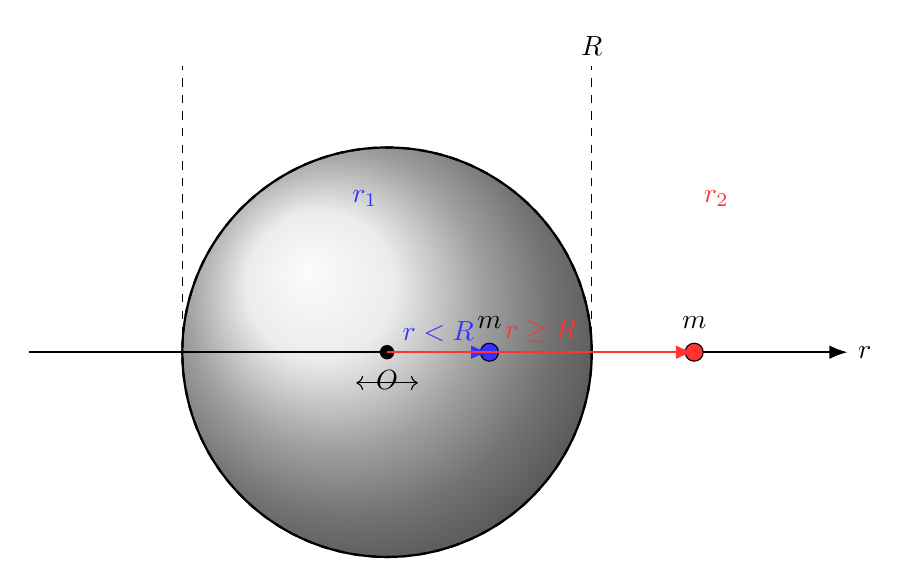
\begin{tikzpicture}[scale=1.3]
  % Sphere with shading
  \shade[ball color=gray!20] (0,0) circle (2);
  \draw[thick] (0,0) circle (2);
  \fill (0,0) circle (2pt) node[below=3pt]{$O$};
  % Radial axis
  \draw[-{Latex},thick] (-3.5,0) -- (4.5,0) node[right]{$r$};
  % Mark R with dashed circle
  \draw[dashed,thick] (0,0) circle (2);
  \draw[dashed] (2,0) -- (2,2.8);
  \draw[dashed] (-2,0) -- (-2,2.8);
  \node[above] at (2,2.8) {$R$};
  % Case r < R
  \coordinate (r1) at (1,0);
  \draw[fill=blue!80] (r1) circle (2.5pt) node[above=5pt]{$m$};
  \draw[-{Latex},blue!80,thick] (0,0) -- (r1) node[midway,above,sloped]{$r < R$};
  \draw[dashed,blue!50] (r1) -- (r1) ++(0,1.5);
  \node[left,blue!80] at (0,1.5) {$r_1$};
  % Case r > R
  \coordinate (r2) at (3,0);
  \draw[fill=red!80] (r2) circle (2.5pt) node[above=5pt]{$m$};
  \draw[-{Latex},red!80,thick] (0,0) -- (r2) node[midway,above,sloped]{$r \geq R$};
  \draw[dashed,red!50] (r2) -- (r2) ++(0,1.5);
  \node[right,red!80] at (3,1.5) {$r_2$};
  % Origin marker
  \draw[<->] (-0.3,-0.3) -- (0.3,-0.3);
\end{tikzpicture}
\end{center}

\section*{Q2. Explore Vesta (10 pts)}
Given: diameter $D = \SI{520}{km}$, so radius $R = \SI{260}{km} = \SI{2.60e5}{m}$, mass $M = \SI{2.67e20}{kg}$.

\textbf{(1) Escape speed:}
\[ v_{\text{esc}} = \sqrt{\frac{2GM}{R}} = \sqrt{\frac{2 \times 6.674 \times 10^{-11} \times 2.67 \times 10^{20}}{2.60 \times 10^5}} = \ans{\SI{370}{m/s}}. \]

\textbf{(2) Orbital period:} For a circular orbit at altitude $h = \SI{15}{km}$ above the surface, the orbital radius is $r = R + h = \SI{2.75e5}{m}$. Using Kepler's third law:
\[ T = 2\pi\sqrt{\frac{r^3}{GM}} = 2\pi\sqrt{\frac{(2.75 \times 10^5)^3}{6.674 \times 10^{-11} \times 2.67 \times 10^{20}}} = 2\pi\sqrt{\frac{2.08 \times 10^{16}}{1.78 \times 10^{10}}} = 2\pi \times 1080 = \ans{\SI{6.79e3}{s} = \SI{1.89}{h}}. \]

\textbf{(3) Reflection:} A spherical model is only marginally useful because Vesta is not spherical—it's an irregular asteroid with significant deviations from sphericity. Real orbits are tricky due to:
\begin{itemize}
  \item Non-uniform mass distribution (density variations)
  \item Irregular shape causing non-central gravitational field
  \item Rotational effects and potential tumbling
  \item Surface features (craters, ridges) that create gravitational anomalies
\end{itemize}
These factors cause orbital perturbations, precession, and instability that a simple spherical model cannot capture.

\section*{Q3. Kepler's law—Pluto's small moons (8 pts)}
Given: Charon orbits at $r_C = \SI{19600}{km}$ with period $T_C = \SI{6.39}{d}$. Two small satellites at $r_1 = \SI{48000}{km}$ and $r_2 = \SI{64000}{km}$.

\textbf{Kepler's third law:} $T^2 \propto r^3$, so $T \propto r^{3/2}$. Scaling from Charon:
\[ \frac{T}{T_C} = \left(\frac{r}{r_C}\right)^{3/2} \quad\Rightarrow\quad T = T_C\left(\frac{r}{r_C}\right)^{3/2}. \]

For $r_1 = \SI{48000}{km}$:
\[ T_1 = 6.39 \times \left(\frac{48000}{19600}\right)^{3/2} = 6.39 \times (2.449)^{3/2} = 6.39 \times 3.83 = \ans{\SI{24.5}{d} = \SI{588}{h}}. \]

For $r_2 = \SI{64000}{km}$:
\[ T_2 = 6.39 \times \left(\frac{64000}{19600}\right)^{3/2} = 6.39 \times (3.265)^{3/2} = 6.39 \times 5.90 = \ans{\SI{37.7}{d} = \SI{905}{h}}. \]

\begin{center}
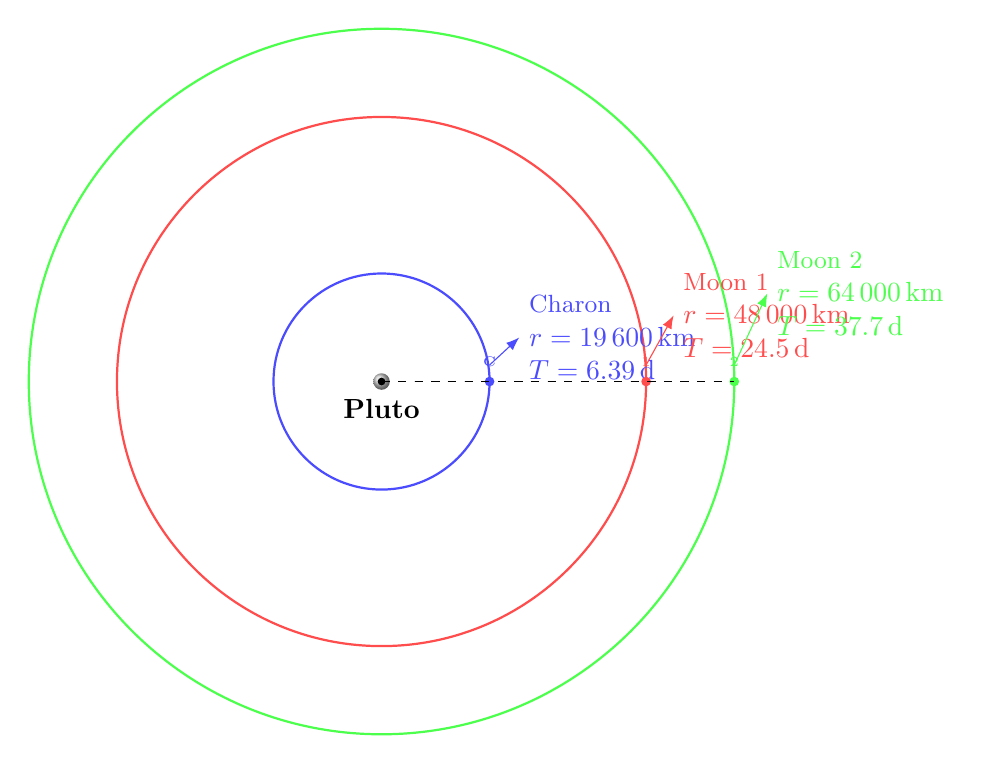
\begin{tikzpicture}[scale=0.7]
  % Pluto at center (larger)
  \shade[ball color=gray!40] (0,0) circle (0.15);
  \fill (0,0) circle (2pt);
  \node[below=3pt] at (0,0) {\textbf{Pluto}};
  % Three orbits with different line styles
  \draw[thick,blue!70] (0,0) circle (1.96);
  \draw[thick,red!70] (0,0) circle (4.8);
  \draw[thick,green!70] (0,0) circle (6.4);
  % Label orbits with arrows
  \draw[-{Latex},blue!70] (1.96,0.3) -- (2.5,0.8);
  \node[right,blue!70,align=left] at (2.5,0.8) {\small Charon\\$r = \SI{19600}{km}$\\$T = \SI{6.39}{d}$};
  \draw[-{Latex},red!70] (4.8,0.3) -- (5.3,1.2);
  \node[right,red!70,align=left] at (5.3,1.2) {\small Moon 1\\$r = \SI{48000}{km}$\\$T = \SI{24.5}{d}$};
  \draw[-{Latex},green!70] (6.4,0.3) -- (7.0,1.6);
  \node[right,green!70,align=left] at (7.0,1.6) {\small Moon 2\\$r = \SI{64000}{km}$\\$T = \SI{37.7}{d}$};
  % Mark moons on orbits
  \fill[blue!70] (1.96,0) circle (2.5pt) node[above=2pt] {\tiny C};
  \fill[red!70] (4.8,0) circle (2.5pt) node[above=2pt] {\tiny 1};
  \fill[green!70] (6.4,0) circle (2.5pt) node[above=2pt] {\tiny 2};
  % Add radial lines
  \draw[dashed,thin] (0,0) -- (1.96,0);
  \draw[dashed,thin] (0,0) -- (4.8,0);
  \draw[dashed,thin] (0,0) -- (6.4,0);
\end{tikzpicture}
\end{center}

\section*{Q4. Gravity and SHM in a straight tunnel (14 pts)}
For a uniform spherical planet of radius $R$ and density $\rho$, the mass inside radius $r$ is $M(r) = \frac{4}{3}\pi r^3\rho$.

\textbf{(2) Gravitational force:} At distance $r$ from the center ($r \leq R$), only the mass inside $r$ contributes:
\[ F(r) = -\frac{GM(r)m}{r^2} = -\frac{G \cdot \frac{4}{3}\pi r^3\rho \cdot m}{r^2} = -\frac{4\pi G\rho m}{3}r. \]
The force is proportional to $r$ and directed toward the center (restoring).

\textbf{(3) Simple harmonic motion:} Newton's second law gives
\[ m\frac{d^2r}{dt^2} = -\frac{4\pi G\rho m}{3}r \quad\Rightarrow\quad \frac{d^2r}{dt^2} = -\frac{4\pi G\rho}{3}r. \]
This is SHM with angular frequency
\[ \omega = \sqrt{\frac{4\pi G\rho}{3}}. \]

\textbf{(4) Period:}
\[ T = \frac{2\pi}{\omega} = 2\pi\sqrt{\frac{3}{4\pi G\rho}} = \sqrt{\frac{3\pi}{G\rho}}. \]

\textbf{(5) Comparison with circular orbit:} For a circular orbit skimming the surface ($r = R$), the orbital speed is $v = \sqrt{GM/R}$ where $M = \frac{4}{3}\pi R^3\rho$. The period is
\[ T_{\text{orbit}} = \frac{2\pi R}{v} = 2\pi R\sqrt{\frac{R}{GM}} = 2\pi\sqrt{\frac{R^3}{G \cdot \frac{4}{3}\pi R^3\rho}} = \sqrt{\frac{3\pi}{G\rho}}. \]
Thus $T = T_{\text{orbit}}$: the tunnel period equals the surface-skimming orbital period.

\textbf{(6) Check:} If density doubles ($\rho \to 2\rho$), then $T = \sqrt{3\pi/(G\rho)} \propto 1/\sqrt{\rho}$, so the period decreases by a factor of $\sqrt{2}$.

\textbf{(1) Drawing:}
\begin{center}
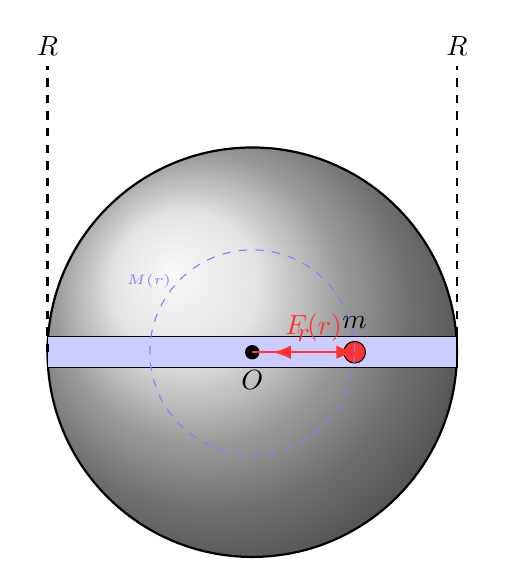
\begin{tikzpicture}[scale=1.3]
  % Planet circle with shading
  \shade[ball color=gray!30] (0,0) circle (2);
  \draw[thick] (0,0) circle (2);
  % Tunnel (diameter) - make it more visible
  \draw[ultra thick,blue!80] (-2,0) -- (2,0);
  \draw[fill=blue!20] (-2,-0.15) rectangle (2,0.15);
  % Center
  \fill (0,0) circle (2pt) node[below=3pt]{$O$};
  % Point at distance r from center
  \coordinate (r) at (1,0);
  \draw[fill=red!80] (r) circle (3pt) node[above=5pt]{$m$};
  \draw[-{Latex},red!80,thick] (0,0) -- (r) node[midway,above,sloped]{$r$};
  % Force vector (restoring, toward center)
  \draw[-{Latex},thick,red!80] (r) -- (0.2,0) node[midway,above]{$F(r)$};
  % Label R
  \draw[dashed,thick] (2,0) -- (2,2.8);
  \draw[dashed,thick] (-2,0) -- (-2,2.8);
  \node[above] at (2,2.8) {$R$};
  \node[above] at (-2,2.8) {$R$};
  % Add mass inside r indicator
  \draw[dashed,blue!50] (0,0) circle (1);
  \node[left,blue!50] at (-0.7,0.7) {\tiny $M(r)$};
\end{tikzpicture}
\end{center}

\section*{Q5. Pendulum in an elevator (10 pts)}
For a pendulum of length $\ell$, the period is $T = 2\pi\sqrt{\ell/g_{\text{eff}}}$, where $g_{\text{eff}}$ is the effective gravitational acceleration in the elevator's reference frame.

\textbf{(1) Cases:}
\begin{itemize}
  \item \textbf{Rest:} $g_{\text{eff}} = g$, so $T_0 = 2\pi\sqrt{\ell/g}$.
  \item \textbf{Accelerating upward at $a$:} In the elevator frame, effective gravity is $g_{\text{eff}} = g + a$, so $T_{\text{up}} = 2\pi\sqrt{\ell/(g+a)}$.
  \item \textbf{Accelerating downward at $a$ (with $a < g$):} Effective gravity is $g_{\text{eff}} = g - a$, so $T_{\text{down}} = 2\pi\sqrt{\ell/(g-a)}$.
\end{itemize}

\textbf{(3) Numerical values:} With $\ell = \SI{0.90}{m}$ and $a = \SI{2.0}{m/s^2}$:
\begin{align*}
T_0 &= 2\pi\sqrt{\frac{0.90}{9.8}} = \ans{\SI{1.90}{s}}, \\
T_{\text{up}} &= 2\pi\sqrt{\frac{0.90}{9.8 + 2.0}} = 2\pi\sqrt{\frac{0.90}{11.8}} = \ans{\SI{1.74}{s}}, \\
T_{\text{down}} &= 2\pi\sqrt{\frac{0.90}{9.8 - 2.0}} = 2\pi\sqrt{\frac{0.90}{7.8}} = \ans{\SI{2.13}{s}}.
\end{align*}
Ranking: $T_{\text{down}} > T_0 > T_{\text{up}}$. The period is longest when accelerating downward (smallest effective $g$).

\textbf{(4) Free fall:} In free fall, $a = g$, so $g_{\text{eff}} = g - g = 0$. The period becomes infinite—the pendulum doesn't oscillate; it floats relative to the elevator.

\begin{center}
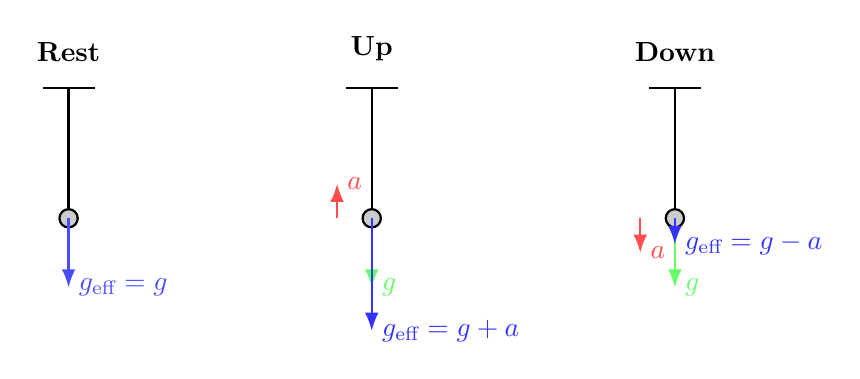
\begin{tikzpicture}[scale=1.1]
  % Case 1: Rest
  \begin{scope}[xshift=-3.5cm]
    % Ceiling
    \draw[thick] (-0.3,0) -- (0.3,0);
    % Pendulum string
    \draw[thick] (0,0) -- (0,-1.5);
    % Bob
    \fill[gray!40] (0,-1.5) circle (3pt);
    \draw[thick] (0,-1.5) circle (3pt);
    % Effective gravity vector
    \draw[-{Latex},thick,blue!70] (0,-1.5) -- (0,-2.3) node[right]{$g_{\text{eff}} = g$};
    \node[above] at (0,0.2) {\textbf{Rest}};
  \end{scope}
  % Case 2: Up
  \begin{scope}
    % Ceiling
    \draw[thick] (-0.3,0) -- (0.3,0);
    % Pendulum string
    \draw[thick] (0,0) -- (0,-1.5);
    % Bob
    \fill[gray!40] (0,-1.5) circle (3pt);
    \draw[thick] (0,-1.5) circle (3pt);
    % Gravity vector
    \draw[-{Latex},thick,green!60] (0,-1.5) -- (0,-2.3) node[right]{$g$};
    % Acceleration vector
    \draw[-{Latex},thick,red!70] (-0.4,-1.5) -- (-0.4,-1.1) node[right]{$a$};
    % Effective gravity
    \draw[-{Latex},thick,blue!80] (0,-1.5) -- (0,-2.8) node[right]{$g_{\text{eff}} = g+a$};
    \node[above] at (0,0.2) {\textbf{Up}};
  \end{scope}
  % Case 3: Down
  \begin{scope}[xshift=3.5cm]
    % Ceiling
    \draw[thick] (-0.3,0) -- (0.3,0);
    % Pendulum string
    \draw[thick] (0,0) -- (0,-1.5);
    % Bob
    \fill[gray!40] (0,-1.5) circle (3pt);
    \draw[thick] (0,-1.5) circle (3pt);
    % Gravity vector
    \draw[-{Latex},thick,green!60] (0,-1.5) -- (0,-2.3) node[right]{$g$};
    % Acceleration vector
    \draw[-{Latex},thick,red!70] (-0.4,-1.5) -- (-0.4,-1.9) node[right]{$a$};
    % Effective gravity
    \draw[-{Latex},thick,blue!80] (0,-1.5) -- (0,-1.8) node[right]{$g_{\text{eff}} = g-a$};
    \node[above] at (0,0.2) {\textbf{Down}};
  \end{scope}
\end{tikzpicture}
\end{center}

\section*{Q6. Van der Waals $\approx$ Hooke near the minimum (8 pts)}
Given potential: $U(r) = U_0\left[\left(\frac{R_0}{r}\right)^{12} - 2\left(\frac{R_0}{r}\right)^6\right]$.

\textbf{(1) Sketch:} The minimum occurs when $dU/dr = 0$. At $r = R_0$, $U(R_0) = U_0(1 - 2) = -U_0$.

\textbf{(2) Conservative force:}
\[ F(r) = -\frac{dU}{dr} = -U_0\left[-12\frac{R_0^{12}}{r^{13}} + 12\frac{R_0^6}{r^7}\right] = 12U_0 R_0^6\left(\frac{R_0^6}{r^{13}} - \frac{1}{r^7}\right). \]

\textbf{(3) Expansion near minimum:} Let $r = R_0 + r'$ with $|r'| \ll R_0$. For small $r'$:
\[ \frac{R_0}{r} = \frac{R_0}{R_0 + r'} = \frac{1}{1 + r'/R_0} \approx 1 - \frac{r'}{R_0} + \cdots. \]

More precisely, expand $F(r)$:
\[ F(R_0 + r') = 12U_0 R_0^6\left[\frac{R_0^6}{(R_0 + r')^{13}} - \frac{1}{(R_0 + r')^7}\right]. \]

Using $(R_0 + r')^{-n} \approx R_0^{-n}(1 - nr'/R_0)$ for small $r'$:
\begin{align*}
F(R_0 + r') &\approx 12U_0 R_0^6\left[\frac{1}{R_0^7}\left(1 - \frac{13r'}{R_0}\right) - \frac{1}{R_0^7}\left(1 - \frac{7r'}{R_0}\right)\right] \\
&= 12U_0 R_0^6 \cdot \frac{1}{R_0^7}\left(-\frac{13r'}{R_0} + \frac{7r'}{R_0}\right) \\
&= -\frac{72U_0}{R_0^2}r'.
\end{align*}
Thus $F \approx -kr'$ with \ans{k = \frac{72U_0}{R_0^2}}.

\textbf{(4) Check:} Units: $[k] = [U_0]/[R_0^2] = \text{J}/\text{m}^2 = \text{N}/\text{m}$ (correct for spring constant). The force is restoring: $F = -kr'$ means $F$ opposes displacement from equilibrium.

\begin{center}
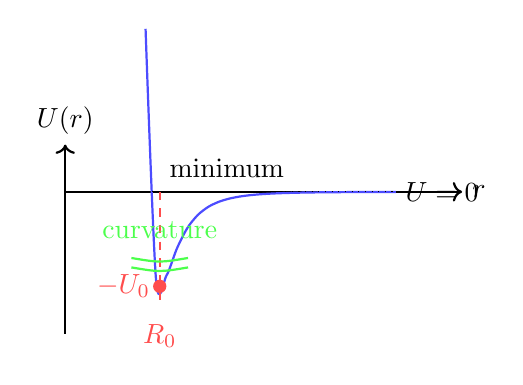
\begin{tikzpicture}[scale=1.2]
  \draw[->,thick] (0,0) -- (4.2,0) node[right]{$r$};
  \draw[->,thick] (0,-1.5) -- (0,0.5) node[above]{$U(r)$};
  % Potential curve (qualitative) - scaled to avoid dimension errors
  \draw[domain=0.85:3.5,smooth,variable=\x,thick,blue!70] plot (\x,{((1/\x)^12 - 2*(1/\x)^6)});
  % Mark R_0 with vertical line
  \draw[dashed,thick,red!70] (1,0) -- (1,-1.2);
  \fill[red!70] (1,-1) circle (2pt);
  \node[below,red!70] at (1,-1.3) {$R_0$};
  \node[left,red!70] at (1,-1) {$-U_0$};
  % Mark minimum point
  \node[above right] at (1,0.05) {minimum};
  % Curvature indicator (parabola near minimum)
  \draw[green!70,thick] (0.7,-0.7) .. controls (1,-0.75) .. (1.3,-0.7);
  \draw[green!70,thick] (0.7,-0.8) .. controls (1,-0.85) .. (1.3,-0.8);
  \node[green!70,above] at (1,-0.6) {curvature};
  % Add zero line
  \draw[dotted] (0.5,0) -- (3.5,0);
  \node[right] at (3.5,0) {$U=0$};
\end{tikzpicture}
\end{center}

\section*{Q7. A moving pulse (9 pts)}
Given: $y(x,t) = \SI{4.20}{m} \cdot e^{-(x+2.00t)^2/(1.20)^2}$.

\textbf{(1) At $t = 0$:} $y(x,0) = \SI{4.20}{m} \cdot e^{-(x/1.20)^2}$. This is a Gaussian pulse centered at $x = 0$ with width $\sim \SI{1.20}{m}$.

\textbf{(2) Rewrite:} $y(x,t) = \SI{4.20}{m} \cdot e^{-(x+2.00t)^2/(1.20)^2} = f(x + 2.00t)$ where $f(u) = \SI{4.20}{m} \cdot e^{-u^2/(1.20)^2}$.

The form $f(x + vt)$ indicates motion in the \textbf{$-x$ direction} with speed \ans{$v = \SI{2.00}{m/s}$}.

\textbf{(3) Center movement:} In $\SI{3.00}{s}$, the center moves $\Delta x = -v \Delta t = -2.00 \times 3.00 = \ans{\SI{-6.00}{m}}$ (to the left).

\begin{center}
\begin{tikzpicture}[scale=1.1]
  % t = 0
  \begin{scope}
    \draw[->,thick] (-2.5,0) -- (4,0) node[right]{$x$ (m)};
    \draw[->,thick] (-2.5,0) -- (-2.5,2.2) node[above]{$y$ (m)};
    % Gaussian pulse at t=0
    \draw[domain=-3:3,smooth,variable=\x,thick,blue!80] plot (\x,{1.8*exp(-(\x)^2/1.44)});
    % Mark center
    \draw[dashed,red!70] (0,0) -- (0,1.8);
    \fill[red!70] (0,1.8) circle (2pt);
    \node[above,red!70] at (0,1.8) {center};
    % Mark width
    \draw[<->,green!70] (-1.2,1.3) -- (1.2,1.3) node[midway,above] {\tiny width $\sim 1.20$ m};
    \node[below] at (0,-0.3) {\textbf{$t = 0$}};
    % Direction arrow
    \draw[-{Latex},thick,red!80] (2.5,1.9) -- (1.5,1.9) node[midway,above]{$-x$ direction};
  \end{scope}
  % t = 3.00 s
  \begin{scope}[yshift=-3.5cm]
    \draw[->,thick] (-9.5,0) -- (3,0) node[right]{$x$ (m)};
    \draw[->,thick] (-9.5,0) -- (-9.5,2.2) node[above]{$y$ (m)};
    % Gaussian pulse at t=3.00s (moved 6 m to the left, so center at x = -6)
    \draw[domain=-9:3,smooth,variable=\x,thick,blue!80] plot (\x,{1.8*exp(-((\x+6)^2)/1.44)});
    % Mark center
    \draw[dashed,red!70] (-6,0) -- (-6,1.8);
    \fill[red!70] (-6,1.8) circle (2pt);
    \node[above,red!70] at (-6,1.8) {center};
    % Mark movement
    \draw[-{Latex},thick,green!70] (0,1.5) -- (-6,1.5) node[midway,above] {\small $\Delta x = -6.00$ m};
    \node[below] at (-6,-0.3) {\textbf{$t = \SI{3.00}{s}$}};
    \node[below] at (-6,-0.6) {center at $x = \SI{-6.00}{m}$};
  \end{scope}
\end{tikzpicture}
\end{center}

\section*{Q8. Wave on a string (10 pts)}
Given: $y(x,t) = A\cos(kx - \omega t + \varphi) = \SI{0.15}{m} \cos(\SI{0.15}{m^{-1}} \cdot x + \SI{1.50}{s^{-1}} \cdot t + 0.25)$.

Note: The signs are $+kx$ and $+\omega t$, so we rewrite as $y = A\cos(kx + \omega t + \varphi)$.

\textbf{(1) Wave speed and direction:}
\[ v = \frac{\omega}{k} = \frac{\SI{1.50}{s^{-1}}}{\SI{0.15}{m^{-1}}} = \ans{\SI{10.0}{m/s}}. \]
The form $\cos(kx + \omega t)$ indicates motion in the \textbf{$-x$ direction} (leftward).

\textbf{(2) At $x = \SI{0.40}{m}$, $t = \SI{5.00}{s}$:}
\begin{align*}
kx + \omega t + \varphi &= 0.15 \times 0.40 + 1.50 \times 5.00 + 0.25 \\
&= 0.06 + 7.50 + 0.25 = 7.810.
\end{align*}
\begin{align*}
y &= \SI{0.15}{m} \cos(7.810) = \ans{\SI{0.007}{m}}, \\
v_y &= \frac{\partial y}{\partial t} = -A\omega\sin(kx + \omega t + \varphi) \\
&= -\SI{0.15}{m} \times \SI{1.50}{s^{-1}} \sin(7.810) = \ans{\SI{-0.225}{m/s}}, \\
a_y &= \frac{\partial^2 y}{\partial t^2} = -A\omega^2\cos(kx + \omega t + \varphi) \\
&= -\SI{0.15}{m} \times (\SI{1.50}{s^{-1}})^2 \cos(7.810) = \ans{\SI{-0.015}{m/s^2}}.
\end{align*}

\section*{Bonus. Wave in different mediums (0--2 pts)}
When you shout near a pond, sound waves in air (a compressional wave with speed $\sim\SI{343}{m/s}$) encounter the water surface. At the air--water interface, most sound energy is \textit{reflected} because of the large impedance mismatch (water's density and bulk modulus are much higher than air's). However, a small fraction \textit{transmits} into water, where sound travels faster ($\sim\SI{1500}{m/s}$) due to water's higher density and bulk modulus. The transmitted wave has a different wavelength ($\lambda_{\text{water}} = v_{\text{water}}/f$) but the same frequency as the incident wave. A detector in water would register this transmitted component, though it would be much weaker than the original sound in air due to the reflection loss at the interface.

\section*{Assistance notes:} LLMs were used as translators and concept explainers. No direct solutions were provided.

\end{document}

